%%%%%%%%%%%%%%%%%%%%%%%%%%%%%%%%%%%%%%%%%
% The Legrand Orange Book
% LaTeX Template
% Version 1.3 (21/8/13)
%
% This template has been downloaded from:
% http://www.LaTeXTemplates.com
%
% Original author:
% Mathias Legrand (legrand.mathias@gmail.com)
%
% License:
% CC BY-NC-SA 3.0 (http://creativecommons.org/licenses/by-nc-sa/3.0/)
%
% Compiling this template:
% This template uses biber for its bibliography and makeindex for its index.
% When you first open the template, compile it from the command line with the
% commands below to make sure your LaTeX distribution is configured correctly:
%
% 1) pdflatex main
% 2) makeindex main.idx -s StyleInd.ist
% 3) biber main
% 4) pdflatex main x 2
%
% After this, when you wish to update the bibliography/index use the appropriate
% command above and make sure to compile with pdflatex several times
% afterwards to propagate your changes to the document.
%
% This template also uses a number of packages which may need to be
% updated to the newest versions for the template to compile. It is strongly
% recommended you update your LaTeX distribution if you have any
% compilation errors.
%
% Important note:
% Chapter heading images should have a 2:1 width:height ratio,
% e.g. 920px width and 460px height.
%
%%%%%%%%%%%%%%%%%%%%%%%%%%%%%%%%%%%%%%%%%

%----------------------------------------------------------------------------------------
%	PACKAGES AND OTHER DOCUMENT CONFIGURATIONS
%----------------------------------------------------------------------------------------

\documentclass[11pt,fleqn]{book} % Default font size and left-justified equations

\usepackage[top=3cm,bottom=3cm,left=3.2cm,right=3.2cm,headsep=10pt,a4paper]{geometry} % Page margins

\usepackage{ctex}
\usepackage{graphics}
\usepackage[lyric]{songs}
\usepackage{xcolor} % Required for specifying colors by name
\definecolor{ocre}{RGB}{243,102,25} % Define the orange color used for highlighting throughout the book

% Font Settings
\usepackage{avant} % Use the Avantgarde font for headings
%\usepackage{times} % Use the Times font for headings
\usepackage{mathptmx} % Use the Adobe Times Roman as the default text font
% together with math symbols from the Sym­bol, Chancery and Com­puter Modern fonts

\usepackage{microtype} % Slightly tweak font spacing for aesthetics
\usepackage[utf8]{inputenc} % Required for including letters with accents
\usepackage[T1]{fontenc} % Use 8-bit encoding that has 256 glyphs

% Bibliography
\usepackage[style=alphabetic,sorting=nyt,sortcites=true,autopunct=true,babel=hyphen,hyperref=true,abbreviate=false,backref=true,backend=biber]{biblatex}
\addbibresource{bibliography.bib} % BibTeX bibliography file
\defbibheading{bibempty}{}

% Index
\usepackage{calc} % For simpler calculation - used for spacing the index letter headings correctly
\usepackage{makeidx} % Required to make an index
\makeindex % Tells LaTeX to create the files required for indexing

%----------------------------------------------------------------------------------------

%----------------------------------------------------------------------------------------
%	VARIOUS REQUIRED PACKAGES
%----------------------------------------------------------------------------------------

\usepackage{titlesec} % Allows customization of titles

\usepackage{graphicx} % Required for including pictures
\graphicspath{{Pictures/}} % Specifies the directory where pictures are stored

\usepackage{lipsum} % Inserts dummy text

\usepackage{tikz} % Required for drawing custom shapes

\usepackage[english]{babel} % English language/hyphenation

\usepackage{enumitem} % Customize lists
\setlist{nolistsep} % Reduce spacing between bullet points and numbered lists

\usepackage{booktabs} % Required for nicer horizontal rules in tables

\usepackage{eso-pic} % Required for specifying an image background in the title page

%----------------------------------------------------------------------------------------
%	MAIN TABLE OF CONTENTS
%----------------------------------------------------------------------------------------

\usepackage{titletoc} % Required for manipulating the table of contents

\contentsmargin{0cm} % Removes the default margin
% Chapter text styling
\titlecontents{chapter}[1.25cm] % Indentation
{\addvspace{15pt}\large\sffamily\bfseries} % Spacing and font options for chapters
{\color{ocre!60}\contentslabel[\Large\thecontentslabel]{1.25cm}\color{ocre}} % Chapter number
{}  
{\color{ocre!60}\normalsize\sffamily\bfseries\;\titlerule*[.5pc]{.}\;\thecontentspage} % Page number
% Section text styling
\titlecontents{section}[1.25cm] % Indentation
{\addvspace{5pt}\sffamily\bfseries} % Spacing and font options for sections
{\contentslabel[\thecontentslabel]{1.25cm}} % Section number
{}
{\sffamily\hfill\color{black}\thecontentspage} % Page number
[]
% Subsection text styling
\titlecontents{subsection}[1.25cm] % Indentation
{\addvspace{1pt}\sffamily\small} % Spacing and font options for subsections
{\contentslabel[\thecontentslabel]{1.25cm}} % Subsection number
{}
{\sffamily\;\titlerule*[.5pc]{.}\;\thecontentspage} % Page number
[] 

%----------------------------------------------------------------------------------------
%	MINI TABLE OF CONTENTS IN CHAPTER HEADS
%----------------------------------------------------------------------------------------

% Section text styling
\titlecontents{lsection}[0em] % Indendating
{\footnotesize\sffamily} % Font settings
{}
{}
{}

% Subsection text styling
\titlecontents{lsubsection}[.5em] % Indentation
{\normalfont\footnotesize\sffamily} % Font settings
{}
{}
{}
 
%----------------------------------------------------------------------------------------
%	PAGE HEADERS
%----------------------------------------------------------------------------------------

\usepackage{fancyhdr} % Required for header and footer configuration

\pagestyle{fancy}
\renewcommand{\chaptermark}[1]{\markboth{\sffamily\normalsize\bfseries #1}{}} % Chapter text font settings
\renewcommand{\sectionmark}[1]{\markright{\sffamily\normalsize\thesection\hspace{5pt}#1}{}} % Section text font settings
\fancyhf{} \fancyhead[LE,RO]{\sffamily\normalsize\thepage} % Font setting for the page number in the header
\fancyhead[LO]{\rightmark} % Print the nearest section name on the left side of odd pages
\fancyhead[RE]{\leftmark} % Print the current chapter name on the right side of even pages
\renewcommand{\headrulewidth}{0.5pt} % Width of the rule under the header
\addtolength{\headheight}{2.5pt} % Increase the spacing around the header slightly
\renewcommand{\footrulewidth}{0pt} % Removes the rule in the footer
\fancypagestyle{plain}{\fancyhead{}\renewcommand{\headrulewidth}{0pt}} % Style for when a plain pagestyle is specified

% Removes the header from odd empty pages at the end of chapters
\makeatletter
\renewcommand{\cleardoublepage}{
\clearpage\ifodd\c@page\else
\hbox{}
\vspace*{\fill}
\thispagestyle{empty}
\newpage
\fi}

%----------------------------------------------------------------------------------------
%	THEOREM STYLES
%----------------------------------------------------------------------------------------

\usepackage{amsmath,amsfonts,amssymb,amsthm} % For including math equations, theorems, symbols, etc

\newcommand{\intoo}[2]{\mathopen{]}#1\,;#2\mathclose{[}}
\newcommand{\ud}{\mathop{\mathrm{{}d}}\mathopen{}}
\newcommand{\intff}[2]{\mathopen{[}#1\,;#2\mathclose{]}}
\newtheorem{notation}{Notation}[chapter]

%%%%%%%%%%%%%%%%%%%%%%%%%%%%%%%%%%%%%%%%%%%%%%%%%%%%%%%%%%%%%%%%%%%%%%%%%%%
%%%%%%%%%%%%%%%%%%%% dedicated to boxed/framed environements %%%%%%%%%%%%%%
%%%%%%%%%%%%%%%%%%%%%%%%%%%%%%%%%%%%%%%%%%%%%%%%%%%%%%%%%%%%%%%%%%%%%%%%%%%
\newtheoremstyle{ocrenumbox}% % Theorem style name
{0pt}% Space above
{0pt}% Space below
{\normalfont}% % Body font
{}% Indent amount
{\small\bf\sffamily\color{ocre}}% % Theorem head font
{\;}% Punctuation after theorem head
{0.25em}% Space after theorem head
{\small\sffamily\color{ocre}\thmname{#1}\nobreakspace\thmnumber{\@ifnotempty{#1}{}\@upn{#2}}% Theorem text (e.g. Theorem 2.1)
\thmnote{\nobreakspace\the\thm@notefont\sffamily\bfseries\color{black}---\nobreakspace#3.}} % Optional theorem note
\renewcommand{\qedsymbol}{$\blacksquare$}% Optional qed square

\newtheoremstyle{blacknumex}% Theorem style name
{5pt}% Space above
{5pt}% Space below
{\normalfont}% Body font
{} % Indent amount
{\small\bf\sffamily}% Theorem head font
{\;}% Punctuation after theorem head
{0.25em}% Space after theorem head
{\small\sffamily{\tiny\ensuremath{\blacksquare}}\nobreakspace\thmname{#1}\nobreakspace\thmnumber{\@ifnotempty{#1}{}\@upn{#2}}% Theorem text (e.g. Theorem 2.1)
\thmnote{\nobreakspace\the\thm@notefont\sffamily\bfseries---\nobreakspace#3.}}% Optional theorem note

\newtheoremstyle{blacknumbox} % Theorem style name
{0pt}% Space above
{0pt}% Space below
{\normalfont}% Body font
{}% Indent amount
{\small\bf\sffamily}% Theorem head font
{\;}% Punctuation after theorem head
{0.25em}% Space after theorem head
{\small\sffamily\thmname{#1}\nobreakspace\thmnumber{\@ifnotempty{#1}{}\@upn{#2}}% Theorem text (e.g. Theorem 2.1)
\thmnote{\nobreakspace\the\thm@notefont\sffamily\bfseries---\nobreakspace#3.}}% Optional theorem note

%%%%%%%%%%%%%%%%%%%%%%%%%%%%%%%%%%%%%%%%%%%%%%%%%%%%%%%%%%%%%%%%%%%%%%%%%%%
%%%%%%%%%%%%% dedicated to non-boxed/non-framed environements %%%%%%%%%%%%%
%%%%%%%%%%%%%%%%%%%%%%%%%%%%%%%%%%%%%%%%%%%%%%%%%%%%%%%%%%%%%%%%%%%%%%%%%%%
\newtheoremstyle{ocrenum}% % Theorem style name
{5pt}% Space above
{5pt}% Space below
{\normalfont}% % Body font
{}% Indent amount
{\small\bf\sffamily\color{ocre}}% % Theorem head font
{\;}% Punctuation after theorem head
{0.25em}% Space after theorem head
{\small\sffamily\color{ocre}\thmname{#1}\nobreakspace\thmnumber{\@ifnotempty{#1}{}\@upn{#2}}% Theorem text (e.g. Theorem 2.1)
\thmnote{\nobreakspace\the\thm@notefont\sffamily\bfseries\color{black}---\nobreakspace#3.}} % Optional theorem note
\renewcommand{\qedsymbol}{$\blacksquare$}% Optional qed square
\makeatother

% Defines the theorem text style for each type of theorem to one of the three styles above
\newcounter{dummy} 
\numberwithin{dummy}{section}
\theoremstyle{ocrenumbox}
\newtheorem{theoremeT}[dummy]{Theorem}
\newtheorem{problem}{Problem}[chapter]
\newtheorem{exerciseT}{Exercise}[chapter]
\theoremstyle{blacknumex}
\newtheorem{exampleT}{Example}[chapter]
\theoremstyle{blacknumbox}
\newtheorem{vocabulary}{Vocabulary}[chapter]
\newtheorem{definitionT}{Definition}[section]
\newtheorem{corollaryT}[dummy]{Corollary}
\theoremstyle{ocrenum}
\newtheorem{proposition}[dummy]{Proposition}

%----------------------------------------------------------------------------------------
%	DEFINITION OF COLORED BOXES
%----------------------------------------------------------------------------------------

\RequirePackage[framemethod=default]{mdframed} % Required for creating the theorem, definition, exercise and corollary boxes

% Theorem box
\newmdenv[skipabove=7pt,
skipbelow=7pt,
backgroundcolor=black!5,
linecolor=ocre,
innerleftmargin=5pt,
innerrightmargin=5pt,
innertopmargin=5pt,
leftmargin=0cm,
rightmargin=0cm,
innerbottommargin=5pt]{tBox}

% Exercise box	  
\newmdenv[skipabove=7pt,
skipbelow=7pt,
rightline=false,
leftline=true,
topline=false,
bottomline=false,
backgroundcolor=ocre!10,
linecolor=ocre,
innerleftmargin=5pt,
innerrightmargin=5pt,
innertopmargin=5pt,
innerbottommargin=5pt,
leftmargin=0cm,
rightmargin=0cm,
linewidth=4pt]{eBox}	

% Definition box
\newmdenv[skipabove=7pt,
skipbelow=7pt,
rightline=false,
leftline=true,
topline=false,
bottomline=false,
linecolor=ocre,
innerleftmargin=5pt,
innerrightmargin=5pt,
innertopmargin=0pt,
leftmargin=0cm,
rightmargin=0cm,
linewidth=4pt,
innerbottommargin=0pt]{dBox}	

% Corollary box
\newmdenv[skipabove=7pt,
skipbelow=7pt,
rightline=false,
leftline=true,
topline=false,
bottomline=false,
linecolor=gray,
backgroundcolor=black!5,
innerleftmargin=5pt,
innerrightmargin=5pt,
innertopmargin=5pt,
leftmargin=0cm,
rightmargin=0cm,
linewidth=4pt,
innerbottommargin=5pt]{cBox}				  
		  

% Creates an environment for each type of theorem and assigns it a theorem text style from the "Theorem Styles" section above and a colored box from above
\newenvironment{theorem}{\begin{tBox}\begin{theoremeT}}{\end{theoremeT}\end{tBox}}
\newenvironment{exercise}{\begin{eBox}\begin{exerciseT}}{\hfill{\color{ocre}\tiny\ensuremath{\blacksquare}}\end{exerciseT}\end{eBox}}				  
\newenvironment{definition}{\begin{dBox}\begin{definitionT}}{\end{definitionT}\end{dBox}}	
\newenvironment{example}{\begin{exampleT}}{\hfill{\tiny\ensuremath{\blacksquare}}\end{exampleT}}		
\newenvironment{corollary}{\begin{cBox}\begin{corollaryT}}{\end{corollaryT}\end{cBox}}	

%----------------------------------------------------------------------------------------
%	REMARK ENVIRONMENT
%----------------------------------------------------------------------------------------

\newenvironment{remark}{\par\vskip10pt\small % Vertical white space above the remark and smaller font size
\begin{list}{}{
\leftmargin=35pt % Indentation on the left
\rightmargin=25pt}\item\ignorespaces % Indentation on the right
\makebox[-2.5pt]{\begin{tikzpicture}[overlay]
\node[draw=ocre!60,line width=1pt,circle,fill=ocre!25,font=\sffamily\bfseries,inner sep=2pt,outer sep=0pt] at (-15pt,0pt){\textcolor{ocre}{R}};\end{tikzpicture}} % Orange R in a circle
\advance\baselineskip -1pt}{\end{list}\vskip5pt} % Tighter line spacing and white space after remark

%----------------------------------------------------------------------------------------
%	SECTION NUMBERING IN THE MARGIN
%----------------------------------------------------------------------------------------

\makeatletter
\renewcommand{\@seccntformat}[1]{\llap{\textcolor{ocre}{\csname the#1\endcsname}\hspace{1em}}}                    
\renewcommand{\section}{\@startsection{section}{1}{\z@}
{-4ex \@plus -1ex \@minus -.4ex}
{1ex \@plus.2ex }
{\normalfont\large\sffamily\bfseries}}
\renewcommand{\subsection}{\@startsection {subsection}{2}{\z@}
{-3ex \@plus -0.1ex \@minus -.4ex}
{0.5ex \@plus.2ex }
{\normalfont\sffamily\bfseries}}
\renewcommand{\subsubsection}{\@startsection {subsubsection}{3}{\z@}
{-2ex \@plus -0.1ex \@minus -.2ex}
{0.2ex \@plus.2ex }
{\normalfont\small\sffamily\bfseries}}                        
\renewcommand\paragraph{\@startsection{paragraph}{4}{\z@}
{-2ex \@plus-.2ex \@minus .2ex}
{0.1ex}
{\normalfont\small\sffamily\bfseries}}

%----------------------------------------------------------------------------------------
%	CHAPTER HEADINGS
%----------------------------------------------------------------------------------------

\newcommand{\thechapterimage}{}
\newcommand{\chapterimage}[1]{\renewcommand{\thechapterimage}{#1}}
\def\thechapter{\arabic{chapter}}
\def\@makechapterhead#1{
\thispagestyle{empty}
{\centering \normalfont\sffamily
\ifnum \c@secnumdepth >\m@ne
\if@mainmatter
\startcontents
\begin{tikzpicture}[remember picture,overlay]
\node at (current page.north west)
{\begin{tikzpicture}[remember picture,overlay]

\node[anchor=north west,inner sep=0pt] at (0,0) {\includegraphics[width=\paperwidth]{\thechapterimage}};

%Commenting the 3 lines below removes the small contents box in the chapter heading
\draw[fill=white,opacity=.6] (1cm,0) rectangle (8cm,-7cm);
\node[anchor=north west] at (1cm,.25cm) {\parbox[t][8cm][t]{6.5cm}{\huge\bfseries\flushleft \printcontents{l}{1}{\setcounter{tocdepth}{2}}}};

\draw[anchor=west] (5cm,-9cm) node [rounded corners=25pt,fill=white,fill opacity=.6,text opacity=1,draw=ocre,draw opacity=1,line width=2pt,inner sep=15pt]{\huge\sffamily\bfseries\textcolor{black}{\thechapter\ ---\ #1\vphantom{plPQq}\makebox[22cm]{}}};
\end{tikzpicture}};
\end{tikzpicture}}\par\vspace*{230\p@}
\fi
\fi
}
\def\@makeschapterhead#1{
\thispagestyle{empty}
{\centering \normalfont\sffamily
\ifnum \c@secnumdepth >\m@ne
\if@mainmatter
\startcontents
\begin{tikzpicture}[remember picture,overlay]
\node at (current page.north west)
{\begin{tikzpicture}[remember picture,overlay]
\node[anchor=north west] at (-4pt,4pt) {\includegraphics[width=\paperwidth]{\thechapterimage}};
\draw[anchor=west] (5cm,-9cm) node [rounded corners=25pt,fill=white,opacity=.7,inner sep=15.5pt]{\huge\sffamily\bfseries\textcolor{black}{\vphantom{plPQq}\makebox[22cm]{}}};
\draw[anchor=west] (5cm,-9cm) node [rounded corners=25pt,draw=ocre,line width=2pt,inner sep=15pt]{\huge\sffamily\bfseries\textcolor{black}{#1\vphantom{plPQq}\makebox[22cm]{}}};
\end{tikzpicture}};
\end{tikzpicture}}\par\vspace*{230\p@}
\fi
\fi
}
\makeatother % Insert the commands.tex file which contains the majority of the structure behind the template

\begin{document}

%----------------------------------------------------------------------------------------
%	TITLE PAGE
%----------------------------------------------------------------------------------------

\begingroup
\thispagestyle{empty}
\AddToShipoutPicture*{\put(6,5){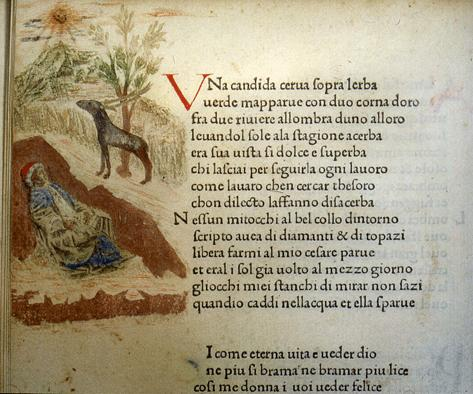
\includegraphics[scale=0.6]{Canzoniere7}}} %
% Image background
\centering
\vspace*{9cm}
\par\normalfont\fontsize{35}{35}\sffamily\selectfont
�豾 (The Song Book)\par % Book title
\vspace*{1cm}
{\Huge �� (ant\_heng)}\par % Author name
\endgroup

%----------------------------------------------------------------------------------------
%	COPYRIGHT PAGE
%----------------------------------------------------------------------------------------

\newpage
~\vfill
\thispagestyle{empty}

\noindent Copyright \copyright\ 2013 \\ % Copyright notice

\noindent \textsc{Published by Publisher}\\ % Publisher

\noindent \textsc{book-website.com}\\ % URL

\noindent Licensed under the Creative Commons Attribution-NonCommercial 3.0 
Unported License (the ``License''). You may not use this file except in 
compliance with the License. You may obtain a copy of the License at 
\url{http://creativecommons.org/licenses/by-nc/3.0}. Unless required 
by applicable law or agreed to in writing, software distributed under 
the License is distributed on an \textsc{``AS IS'' BASIS, WITHOUT WARRANTIES 
OR CONDITIONS OF ANY KIND}, either express or implied. See the License 
for the specific language governing permissions and limitations under 
the License.\\ % License information

\noindent \textit{First printing, March 2013} % Printing/edition date

%----------------------------------------------------------------------------------------
%	TABLE OF CONTENTS
%----------------------------------------------------------------------------------------

\chapterimage{chapter_head_1.pdf} % Table of contents heading image

\pagestyle{empty} % No headers

\tableofcontents % Print the table of contents itself

\cleardoublepage % Forces the first chapter to start on an odd page so it's on the right

\pagestyle{fancy} % Print headers again

%----------------------------------------------------------------------------------------
%	CHAPTERS
%----------------------------------------------------------------------------------------
\songcolumns{1}
\setlength\baselineadj{5pt plus 1pt minus 0pt}

\chapterimage{chapter_head_2.pdf} % Chapter heading image
\songchapter{H}

%%%%%%%%%%%%%%%%%%%%%%%%%%%%%
\songsection{�����}	\index{H!humage}

%%%%%%%%%%%%%%%%%%%
\subsection{���˶��и�С���, �ҵIJ������ʮһ����}

\begin{figure}[htp]
	\begin{center}
	  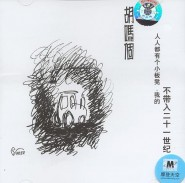
\includegraphics[scale = 0.80]{h/humage/renrendouyou}
	  \label{fig:renrendouyou}
	\end{center}
\end{figure}

\begin{songs}{}
  \beginsong{������������}[index={������������}]
	���³���ɭ��	\\
	��������֦����	\\
	�Լ�������	\\
	�Լ����ֵ�	\\
	��ϲȵ����	\\
	���𿵣��	\\
	����ӥ��С��	\\
	�滨����ú	\\
	�Ի�ȡ��ֻ���Ӷ���	\\
	\vspace{2ex}
	����ס��һ���ֵֹ�û�ж�����Ļ���	\\
	��˵�������¸�������ʵû������	\\
	���ó�һ��д�˺ܶ��ֵ���ϰ�����ҿ�	\\
	�ַ�һЩ��̫�����ܳ��ĸ������	\\
	��˵��������������	\\
	��˵����������	\\
	��ȴҪ��Ц�ݵ���ƨ�������������	\\
	���ᵽ��αʲô��	\\
	��˵��һЩ���еĻ���	\\
	�ö���Ҷ�����̫��	\\
	ֻ��ǸǸ��ǸǸ��˵	\\
	�����˵���� \hspace{5mm} �����ʵ��˵����	\\
	�����˵���� \hspace{5mm} �����ʵ��˵����	\\
	�����˵���� \hspace{5mm} �����ʵ��˵����	\\
	�����˵���� \hspace{5mm} �����ʵ��˵����	\\
	\vspace{2ex}
	�ݶ��ϵ���ֻ��è	\\
	���и��� \hspace{5mm} ����̨	\\
	���Ա���������еĻ�������˯��	\\
	�������Ȣ���� \hspace{5mm} ҡ��һ�� \hspace{5mm} �Ͻ�ȥ	\\
	����һ�������С��¥	\\
	�ͺ���ոǵ��·�	\\
	�Ҿ��������������˹�ȥ	\\
	���ŵĴ��ݸ���һ����ֽ	\\
	˵ \hspace{5mm} ��ëǮһλ	\\
	�����ҵ���ؿ�����	\\
% 	�����ҵ���ؿ�����	\\
% 	�����ҵ���ؿ�����	\\
% 	�����ҵ���ؿ����ҵ���ؿ�����	\\
% 	�����ҵ���ؿ����ҵ������ؿ�����	\\
% 	�����ҵ���ؿ�����ؿ�����	\\
% 	�����ҵ���ؿ�����	\\
% 	�����ҵ���ؿ����ҵ���ؿ�����	\\
% 	�����ҵ�����ҵ���ؿ�����	\\
% 	�����ҵ���ؿ����ҵ���ؿ�����	\\
% 	�����ҵ�����ҵ��ҵ���ؿ�����	\\
% 	�����ҵ���ؿ����ҵ���ؿ�����	\\
% 	�����ҵ���ؿ����ҵ���ؿ�����	\\
% 	�����ҵ�����ҵ���ؿ�����	\\
% 	�����ҵ�����ҵ���ؿ�����	\\
% 	�����ҵ������ؿ�����	\\
% 	�����ҵ������ؿ�����	\\    
  \endsong
  
  \beginsong{���ĵ��ڻ�26·�����ҵ�������������}[index={���ĵ��ڻ�26·�����ҵ�������������}]
	���Ӽ仹�з�϶	\\
	һЩ���������߱�����	\\
	���ǰ칫��	\\
	ǽ�������ƶȱ� \hspace{5mm} �빤���й�	\\
	��ҲŲ��ᵽ��̫��	\\
	�������������	\\
	������Ȼῴ�����ǵ�Ůͬ��	\\
	���ǻ�֦��չ �����Լ�����	\\
	�����Ƕ�����ʵ��̫��	\\
	��֪���ҵİ칫���Ǽ�ֵ�������	\\
	��֪��ϴ�ּ�����ֱ�߾������3��Զ��	\\
	��֪���Ҷ����ʯӢ��ÿ����20����	\\
	��֪�� \hspace{5mm} ��֪��	\\
	����Щ����ʵ����������	\\
	\vspace{2ex}
	��֪ʲôʱ���ҿ�ʼ�����ڴ�绰	\\
	�������ǵ绰��	\\
	��ʱ�� \hspace{5mm} ������ſ������	\\
	ժ����Ͳ�Ҿͻ��ੲ���	\\
	����Ҹ�����һ��	\\
	�Է��Ǹ�Ů��	\\
	��˵����Խ�������	\\
	(...?) �ſڼ�	\\
	�����˷� \hspace{5mm} ��������	\\
	\vspace{2ex}
	�����µ绰�����˸��绰 \hspace{5mm} ���Ǹ�Ů�� \\
	��˵��Ҫ������(?) \hspace{5mm} ��˵���������Ϳ� \\
	��˵��������ǧ���� \hspace{5mm} �����ǿ�	\\
	��˵������Ļ��Ǽٵ� \hspace{5mm} ���Ͳ�����	\\
	\vspace{2ex}
	β���ϵ�������һ����һ��	\\
	����д�˷ݴ�ְ����	\\
	�� \hspace{5mm} ˵��ȥ������	\\
	������ \hspace{5mm} Ϊ���Ƕ���һ������	\\
	���ǿڿ�����Ϊ���ǵ������ߵ�����ף�� \hspace{5mm} ��ʹӹ��	\\
	�������м����˴��ŷ��W�˽���	\\
	����������	\\
	��ÿ�춼���ڼ�����ϰ��°�	\\
	���ﴧ����Ʊ	\\
	���ĵ��ڻ�26·	\\
	�� \hspace{5mm} ���컹���Լ��Ҹ�Ů����ȥ��	\\
	�⿴���˵�	\hspace{5mm} Ҳ������˼	\\  
  \endsong
\end{songs}
\songchapter{L}

%%%%%%%%%%%%%%%%%%%%%%%%%%%%%
\songsection{罗大佑}	\index{L!luodayou}

%%%%%%%%%%%%%%%%%%%
\subsection{未来的主人翁}

\begin{figure}[htp]
	\begin{center}
	  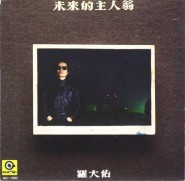
\includegraphics[scale = 0.80]{l/luodayou/weilaidezhurenweng}
% 	  \caption[labelInTOC]{未来的主人翁}
	  \label{fig:weilaidezhurenweng}
	\end{center}
\end{figure}

\begin{songs}{}
  \beginsong{未来的主人翁}[index={未来的主人翁}]
	你走过林立的高楼大厦穿过那些拥挤的人	\\
	望着一个现代化的都市泛起一片水银灯	\\
	突然想起了遥远的过去未曾实现的梦	\\
	曾经一度人们告诉你说你是未来的主人翁	\\
	\vspace{2ex}
	在人潮汹涌的十字路口每个人在痴痴地等	\\
	每个人的眼睛都望着那象征命运的红绿灯	\\
	在红橙黄绿的世界里你这未来的主人翁	\\
	在每一张陌生的面孔里寻找儿时的光荣	\\
	\vspace{2ex}
	每一个今天来到世界的婴孩	\\
	张大了眼睛摸索着一个真心的关怀	\\
	每一个来到世界的生命在期待	\\
	因为我们改变的世界将是他们的未来	\\
	\vspace{2ex}
	别以为我们的孩子们太小他们什么都不懂	\\
	我听到无言的抗议在他们悄悄的睡梦中	\\
	我们不要一个被科学游戏污染的天空	\\
	我们不要被你们发明变成电脑儿童	\\
	\vspace{2ex}
	每一个今天来到世界的婴孩	\\
	张大了眼睛摸索着一个真心的关怀	\\
	每一个来到世界的生命在期待	\\
	因为我们改变的世界将是他们的未来	\\
	\vspace{2ex}
	有一天孩子们会告诉他们后代你们要守规矩	\\
	格言象玩具风筝在风里飘来飘去	\\
	当未来的世界充满了一些陌生的旋律	\\
	你或许会想起现在这首古老的歌曲	\\
	\vspace{2ex}
	飘来飘去 \hspace{5mm} 就这么飘来飘去	\\
	飘来飘去 \hspace{5mm} 就这么飘来飘去	\\
	飘来飘去 \hspace{5mm} 就这么飘来飘去	\\
	飘来飘去 \hspace{5mm} 就这么飘来飘去	\\
	飘来飘去 \hspace{5mm} 就这么飘来飘去	\\
	飘来飘去 \hspace{5mm} 就这么飘来飘去	\\
	飘来飘去 \hspace{5mm} 就这么飘来飘去	\\
	飘来飘去 \hspace{5mm} 就这么飘来飘去	\\
	飘来飘去 \hspace{5mm} 就这么飘来飘去	\\
	飘来飘去 \hspace{5mm} 就这么飘来飘去	\\
	飘来飘去 \hspace{5mm} 就这么飘来飘去	\\
	飘来飘去 \hspace{5mm} 就这么飘来飘去	\\
	\vspace{2ex}	
	我们不要一个被科学游戏污染的天空	\\
	我们不要一个被现实生活超越的时空	\\
	我们不要一个越来越远模糊的水平线	\\
	我们不要一个越来越近沉默的春天	\\
	我们不要被你们发明变成电脑儿童	\\
	我们不要被你们忘怀变成钥匙儿童	\\
	\vspace{2ex}
	我们需要阳光青草泥土开阔的蓝天	\\
	我们不要红色的污泥塑成红色的梦魇	\\
  \endsong
\end{songs}


\songchapter{S}

%%%%%%%%%%%%%%%%%%%%%%%%%%%%%
\songsection{������Ƭ}	\index{S!shengyinsuipian}

%%%%%%%%%%%%%%%%%%%
\subsection{�����ĵ�������}

\begin{figure}[htp]
	\begin{center}
	  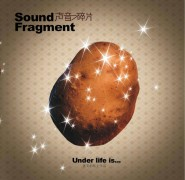
\includegraphics[scale = 0.80]{s/youmei}
% 	  \caption[labelInTOC]{�����ĵ�������}
	  \label{fig:youmei}
	\end{center}
\end{figure}

\begin{songs}{}
  \beginsong{�����ĵ�������}[index={�����ĵ�������}]
	�Ѹ�������ҹ��	\\
	�ѵ�·������ͷ	\\
	�ѹ�ʵ��������	\\
	�ѷ��軹�����	\\
	ʣ�µģ�����������	\\
	���ݵ���صø���	\\
	���ͷ��ҵ�һ��	\\
	�������ĵ�������	\\
	����ѽ��ѽ��ѽ	\\
	ֻҪ����Զ���տ�	\\
	����ѽ��ѽ��ѽ	\\
	�ε��˷��ĵIJ�ԭ	\\
	\vspace{2ex}
	�మ�ɣ�����һɢ������	\\
	��ʧȥ�IJ�����ͯ��	\\
	��ʱ���þ����ഺ	\\
	�������������ڴ�����ܻ�	\\
	����ѽ��ѽ��ѽ	\\
	ֻҪ����Զ���տ�	\\
	����ѽ��ѽ��ѽ	\\
	�ε��˷��ĵIJ�ԭ	\\
	\vspace{2ex}
	����ѽ��ѽ��ѽ	\\
	ֻҪ����Զ���տ�	\\
	����ѽ��ѽ��ѽ	\\
	�ε��˷��ĵIJ�ԭ	\\
  \endsong
  
  \beginsong{��ʱ��������ʢ����}[index={��ʱ��������ʢ����}]
	����ãȻ������	\\
	�Ѿ������˱�ϲ	\\
	�����ںӵ����� Ŀ����ʧ	\\
	��΢���Ļƻ���	\\
	���˿�ʼ������	\\
	�貽�����Ļ��� ��ô����	\\
	��������˵�����	\\
	��˵ý���	\\
	������ȥѡ�� ���Ѿ���	\\
	��ʱ��������ʢ����	\\
	��Ⱥ�������	\\
	������������	\\
	������ȴ��ô����	\\
	\vspace{2ex}
	����ǻ��ֱ���	\\
	Ψһ��ʵ���˿�	\\
	���ȵ��µ����� �����΢Ц	\\
	û���˵õ�����	\\
	û����ѡ���뿪	\\
	�����ŵ���հ� һƶ��ϴ	\\
	��ʱ��������ʢ����	\\
	�̻���������	\\
	���ݵIJ��� ����Ⱥ��ѣ	\\
	��ʱ���޾���������	\\
	�������糾��	\\
	����Զȥ����Ϣ	\\
	�������� ��������	\\
	�������� ��������	\\
	������ ��������	\\
  \endsong
\end{songs}
\songchapter{W}

%%%%%%%%%%%%%%%%%%%%%%%%%%%%%
\songsection{���������õ�}	\index{W!wannengqingnianlvdian}

%%%%%%%%%%%%%%%%%%%
\subsection{���������õ�}

\begin{figure}[htp]
	\begin{center}
	  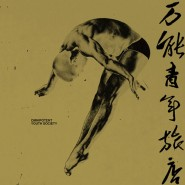
\includegraphics[scale = 0.80]{w/wanneng}
% 	  \caption[labelInTOC]{���������õ�}
	  \label{fig:wanneng}
	\end{center}
\end{figure}

\begin{songs}{}
  \beginsong{������������е��ù�}[index={������������е��ù�}]
  ��Щ�����������˰�	\\
  ��Ϊ�Ѿ� 	\\
  ��Ϥ���ƺ������Ƣ��	\\ 
  �Ͳ����Ի� 	\\
  �Ͳ����˽��Լ������������	\\ 
  ÿ��ֻ�� \\
  ��΢�紵�������ͻ�̸��	\\ 
  \vspace{2ex}
  ���Ǵ�������Ҫ¥��	\\ 
  ֻ�д��� 	\\
  ��һ�н������ξ�	\\
  ���������˳� 	\\
  ����������еľƹ� 	\\
  �ഺ�������ƺ�����Ӧ�� 	\\
  �����ɢ��δ�� 	\\
  ֻ����裬������̹��	\\
  \vspace{2ex}
  �ڿ�ѧ��ơ�ƶ�����	\\ 
  ������ҹ�� 	\\
  ���Ƕ�ʧ���ļ� \\
  �̻�֮�п�ʼ \\
  ����������еľƹ�	\\ 
  �޷�����Զ���ĺ��� 	\\
  Ұ�IJ����ĵƻ� 	\\
  ˲����û�ڰ�������	\\
  \endsong
\end{songs}

%%%%%%%%%%%%%%%%%%%%%%%%%%%%%
\songsection{������}	\index{W!wutiaoren}


\songchapter{X}

%%%%%%%%%%%%%%%%%%%%%%%%%%%%%
\songsection{小河}	\index{X!xiaohe}

%%%%%%%%%%%%%%%%%%%
\subsection{单曲}

\begin{songs}{}
  \beginsong{男厕女厕中间的小房子}[index={男厕女厕中间的小房子}]
    嘿 知道吗 厕所也可以承包了	\\
	去吧 承包一个厕所吧	\\		
	和你的爱人住在男厕女厕中间的小房子里	\\
	去吧 承包一个厕所吧	\\
	你们会有一个和所有家庭一样的家庭	\\
	那里也会飘出让路人快步的菜香	\\
	那里也会生长和爱人入梦的温暖	\\
	你们会有一个和所有孩子一样的孩子	\\
	他一点也不自卑 会叫很多小朋友回来玩	\\
	骄傲的告诉他们 我们家上厕所 不用排队	\\
	他一点也不自卑 像所有孩子一样有一个伟大的理想	\\
	他说长大了以后要盖一个全世界最大最豪华的厕所给妈妈	\\
	他一点也不自卑 像所有孩子一样有一个伟大的理想	\\
	他说长大了以后要建一个全世界最大最豪华的厕所给妈妈	\\
	到那时候 全世界的人来上厕所 都不用排队	\\
  \endsong
\end{songs}

%%%%%%%%%%%%%%%%%%%
\subsection{飞的高的鸟不落在跑不快的牛的背上}

\begin{songs}{}
  \beginsong{丢失了梦的清晨}[index={丢失了梦的清晨}]
		呀咿呀儿呀咿呀咿呀儿	\\
		我害怕这没有尽头的梯子	\\
		因为我没有勇气去选择	\\
		简单和复杂哪个更痛苦	\\
		白痴和骗子哪个更幸福	\\
		因为我没有勇气去选择	\\
		简单和复杂哪个更痛苦	\\
		白痴和骗子哪个更幸福	\\
		因为我没有勇气去选择	\\
		时间不犹豫的在旋转	\\
		真理也会慢慢变谎言	\\
		总有一天你会离它不再远	\\
		你看它不远	\\
		问题的答案就是问题	\\
		证据的疑点就是证据	\\
		此刻的幸福是你在痛苦里	\\
		你在我怀里	\\
		你在我怀里	\\
		窗把风送来的夜里	\\
		孩子哭干了眼泪	\\
		窗把风送来的夜里	\\
		窗把风送来的夜里	\\
		孩子哭干了眼泪	\\
		孩子哭干了眼泪	\\
		窗把风送来的夜里	\\
		孩子哭干了眼泪	\\
		窗把风送来的夜里	\\
		孩子哭干了眼泪	\\
  \endsong
\end{songs}


%%%%%%%%%%%%%%%%%%%%%%%%%%%%%
\songsection{许巍}	\index{X!xuwei}

%%%%%%%%%%%%%%%%%%%
\subsection{在别处}

\begin{figure}[htp]
	\begin{center}
	  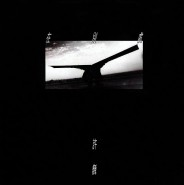
\includegraphics[scale = 0.80]{x/xuwei/zaibiechu}
% 	  \caption[labelInTOC]{在别处}
	  \label{fig:zaibiechu}
	\end{center}
\end{figure}

\begin{songs}{}
  \beginsong{水妖}[index={水妖}]
  	这冬天充满阳光 可我依然迷茫		\\
	我听到你的歌声 随风飘荡	\\
	\vspace{2ex}
	你站在水的中央 让我充满幻想	\\
	你让我进入水底 长发会永远不脏	\\
	这诱惑让我向往 这歌声给我幻想	\\
	我却总回头 留恋岸上风光	\\
	\vspace{2ex}
	这夏天没有阳光 我还站在岸上	\\
	河水已经干枯 不再流淌	\\
	听不到你的歌声 只有风声在响	\\
	看不到你的身影 今昔梦在何方	\\
	无所谓什么坚强 无所谓什么悲伤	\\
	我从来都是这样 没有方向	\\
  \endsong
\end{songs}

%%%%%%%%%%%%%%%%%%%
\subsection{珍藏许巍作品全集}

\begin{figure}[htp]
	\begin{center}
	  
\includegraphics[scale = 0.80]{x/xuwei/zhencang}
% 	  \caption[labelInTOC]{珍藏许巍作品全集}
	  \label{fig:xuweizhencang}
	\end{center}
\end{figure}

\begin{songs}{}
  \beginsong{两天}[index={两天}]
	我还是飞不起来 \hspace{5mm} 依然需要等待	\\
	你就这样离开 \hspace{5mm} 带着所有伤害	\\
	秋天还是秋天 \hspace{5mm} 依然美丽凄凉	\\
	还是飘飘荡荡 \hspace{5mm} 依然充满幻想	\\
	\vspace{2ex}
	我想飞 \hspace{5mm} 还是飞不起来	\\
	我想飞 \hspace{5mm} 在每个想你的秋天	\\
	我想飞 \hspace{5mm} 在歌声响起的夜晚	\\
	\vspace{2ex}
	我看到我的身边 \hspace{5mm} 他们都比我美	\\
	我看到我的身后 \hspace{5mm} 时间都已枯萎	\\
	我想起昨天 \hspace{5mm} 曾吻遍的身体	\\
	我想起从我身边 \hspace{5mm} 再次出走的你	\\
	\vspace{2ex}
	我想飞 \hspace{5mm} 还是飞不起来	\\
	我想飞 \hspace{5mm} 在每个想你的秋天	\\
	我想飞 \hspace{5mm} 在歌声响起的夜晚	\\
	\vspace{2ex}
	我只有两天 \hspace{5mm} 我从没有把握	\\
	一天用来出生 \hspace{5mm} 一天用来死亡	\\
	我只有两天 \hspace{5mm} 我从没有把握	\\
	一天用来希望 \hspace{5mm} 一天用来绝望	\\
	我只有两天 \hspace{5mm} 每天都在幻想	\\
	一天用来想你 \hspace{5mm} 一天用来想我	\\
	我只有两天 \hspace{5mm} 我从没有把握	\\
	一天用来路过 \hspace{5mm} 另一天还是路过 	\\
  \endsong
\end{songs}

\songchapter{Z}

%%%%%%%%%%%%%%%%%%%%%%%%%%%%%
\songsection{������}	\index{Z!zhouyunpeng}

%%%%%%%%%%%%%%%%%%%
\subsection{��Ĭ���յĺ���}

\begin{figure}[htp]
	\begin{center}
	  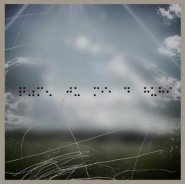
\includegraphics[scale = 0.80]{z/zhouyunpeng/chenmorumi}
% 	  \caption[labelInTOC]{��Ĭ���յĺ���}
	  \label{fig:chenmorumi}
	\end{center}
\end{figure}

\begin{songs}{}
  \beginsong{������ij���ڳ�һ�����˵ĸ�}[by={�������װ�}, index={������ij���ڳ�һ�����˵ĸ�}]
	�����뿪�Ǽ������ķ���	\\
	���Ķ��ѵ�����	\\
	ֻʣ��ij���Լ�����������	\\
	���Ѻ���	\\
	���������ڳ�һ�����˵ĸ�	\\
	\vspace{2ex}
	������������һ���ƻ�	\\
	�����ˮ��Խ��Խ����	\\
	�ӱߵ�ˮ��æ�Ž������	\\
	һƬ������	\\
	������һ�����ֵļ�ͥ	\\
	�����ǵļ��Ѿ���Ȼ�޴�	\\
	���ǵļҺ͵���������һ��	\\
	����Ұ�����������������	\\ 
  \endsong
\end{songs}

%%%%%%%%%%%%%%%%%%%
\subsection{�����}

\begin{figure}[htp]
	\begin{center}
	  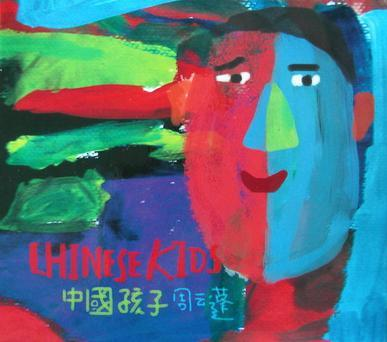
\includegraphics[scale = 0.50]{z/zhouyunpeng/zhongguohaizi}
% 	  \caption[labelInTOC]{�����}
	  \label{fig:zhongguohaizi}
	\end{center}
\end{figure}

\begin{songs}{}
  \beginsong{����}[index={����}]
	һ������������	\\
	�����Ƽ�	\\
	�Ͽ����������	\\
	�¼������ҵĵ�	\\
	���첻������ʳ	\\
	���첻�ظǷ���	\\
	\vspace{2ex}
	���ס��������Ƽ�	\\
	�Ͽ����������	\\
	�¼������ҵĵ�	\\
	���첻������ʳ	\\
	���첻�ظǷ���	\\
	\vspace{2ex}
	���Ǿ�ס���Ʋ�������޻���	\\
	�������޻���͵͵�غȾ�	\\
	��������һ�Ÿ�ɽ	\\
	��������һ��ƽԭ	\\
	��������һ�ź���	\\
	��������һ��ɳ̲	\\
	���ǵ�������һֻˮͰ	\\
	����ȥ�տյ���	\\
	������װ����ˮ	\\
	����ȥ�տյ���	\\
	������װ����ˮ	\\
	\vspace{2ex}
	�����Ƽ�	\\
	�Ͽ����������	\\
	�¼������ҵĵ�	\\
	���첻������ʳ	\\
	���첻�ظǷ���	\\
	\vspace{2ex}
	���ס��������Ƽ�	\\
	�Ͽ����������	\\
	�¼������ҵĵ�	\\
	���첻������ʳ	\\
	���첻�ظǷ���	\\
  \endsong
\end{songs}
%%%%%%%%%%%%%%%%%%%
\subsection{ţ����ɽ}

\begin{figure}[htp]
	\begin{center}
	  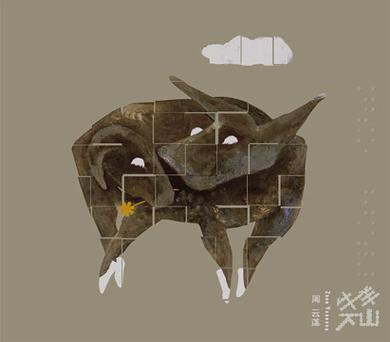
\includegraphics[scale = 0.50]{z/zhouyunpeng/niuyangxiashan}
% 	  \caption[labelInTOC]{ţ����ɽ}
	  \label{fig:niuyangxiashan}
	\end{center}
\end{figure}

\begin{songs}{}
  \beginsong{����˵���İ���}[index={����˵���İ���}]
	�廨��������� \hspace{5mm} ţ��Ҳ��ɽ�	\\
	�������Լ��ķ��Ӻ����� \hspace{5mm} �������	\\ 
	�⿪��ĺ�Ǵ� \hspace{5mm} ��һ��ѩ����	\\ 
	���������е�ˮ \hspace{5mm} ���������е���	\\ 
	û�д����ŵ� \hspace{5mm} û������;��	\\ 
	���ǵ�ľ�������� \hspace{5mm} ˵�Ҹ�������	\\ 
	�����װ�����ѽ \hspace{5mm} �����װ��Ľ�ѽ	\\ 
	��������Ļʺ� \hspace{5mm} �����Ե�С�ײ�	\\ 
	
	���ӿ쵽ͷ�� \hspace{5mm} ����Ҳ��͸��	\\ 
	�������һ���ո�Է� \hspace{5mm} �Ӵ˳����ƺ�	\\ 
	��ȥ���δ�� \hspace{5mm} ��ȥ�ҵ�δ��	\\ 	
	����ֻ���ڱ˴˵��ξ��� \hspace{5mm} ��õ��ǻ�	\\ 
	�ǻ������δ�� \hspace{5mm} �ǻ����ҵ�δ��	\\ 
	�ǻ���ˮ��������� \hspace{5mm} ð�������ڴ�	\\ 
	�ڴ��������˵��� \hspace{5mm} �ڴ����õ��˵���	\\ 
	�ڴ����ǵ���긽�� \hspace{5mm} ���»���	\\ 
	���»��� \hspace{5mm} ���»���	\\ 
  \endsong
\end{songs}
%%%%%%%%%%%%%%%%%%%%%%%%%%%%%
\songsection{֣�ǻ�}	\index{Z!zhengzhihua}

%%%%%%%%%%%%%%%%%%%
\subsection{���۵Ĺ���}

\begin{figure}[htp]
	\begin{center}
	  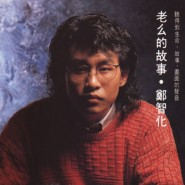
\includegraphics[scale = 0.80]{z/laoyao}
% 	  \caption[labelInTOC]{��������}
	  \label{fig:laoyao}
	\end{center}
\end{figure}

\begin{songs}{}
  \beginsong{���۵Ĺ���}[index={���۵Ĺ���}]
	��ɫ��ú�� \hspace{5 mm} ��ɫ����	\\
	�����ڿ��ﲻ�ϵ���	\\
	����������һ��	\\
	���ݵ����� \hspace{5 mm} ��ǿ����	\\
	������ʲô�Ҳ���	\\
	���в����ҵ���	\\
	\vspace{2ex}
	�����ķ��ݡ���������	\\
	����ı��ز�����	\\
	�����Dz�����	\\
	�����ļ¶������˵ľ�	\\
	���ֵ�����૵�˵	\\
	�������������	\\
	\vspace{2ex}
	ͨ���ӿڵ���һ��·	\\
	����������Ψһ�ķ���	\\
	������ģ���ĽŲ���	\\
	����������һ�ε���	\\
	˭˵�軵�ĺ��Ӳ���	\\
	���ڱ��緢������һ˲��	\\
	��ˮ�Ⱥ�������	\\
	��������û�Ŀ������	\\
	\vspace{2ex}
	��û�Ŀ������û���ҵ���	\\
	��û�Ŀ����û����Ц��	\\
	���յ�ֽǮ�ڿ�����ҷ�	\\
	��ȥ�Ļ��� Ĩ��ȥ���˺�	\\
	�󹤵Ķ��� ������������	\\	
	���ܵ��� ���Ҹ���ε���	\\	
	\vspace{2ex}	
	�������������ִ�ս��	\\
	�ҵõ���һ��ȴʧȥ���Լ�	\\
	�ٶ����Ҳ�������	\\
	������ú�������˻ҽ�	\\
	������˱������ûʧȥ������	\\
	���е��˱�������ûȴʧȥ�����	\\
	��û�Ŀ������û���ҵ���	\\
	��û�Ŀ����û����Ц��	\\
	���ӵ���������һ������	\\
	����Ĺ��޺δ���������	\\
	�ɳ�����������������֪��	\\
	����ļ�������ȥ�ĵط�	\\
  \endsong
\end{songs}


%------------------------------------------------

%----------------------------------------------------------------------------------------
%	BIBLIOGRAPHY
%----------------------------------------------------------------------------------------

\chapter*{�����}
\addcontentsline{toc}{chapter}{\textcolor{ocre}{Bibliography}}
\section*{�鼮}
%\printbibliography[heading=bibempty,type=book]
\section*{����}
%\printbibliography[heading=bibempty,type=article]

%----------------------------------------------------------------------------------------
%	INDEX
%----------------------------------------------------------------------------------------

\cleardoublepage
\setlength{\columnsep}{0.75cm}
\addcontentsline{toc}{chapter}{\textcolor{ocre}{Index}}
\printindex

%----------------------------------------------------------------------------------------

\end{document}
